\documentclass[a4paper]{article}
%\documentclass[8pt]{report}
%%%%%%%% CREATE DOCUMENT STRUCTURE %%%%%%%%
%% Language and font encodings
\usepackage[english]{babel}
\usepackage[utf8x]{inputenc}
\usepackage[T1]{fontenc}

%\usepackage{subfig}

%% Sets page size and margins
\usepackage[a4paper,top=3cm,bottom=2cm,left=2cm,right=2cm,marginparwidth=1.75cm]{geometry}

%% Useful packages
\usepackage{amsmath}
\usepackage{graphicx}
\usepackage[colorinlistoftodos]{todonotes}
\usepackage[colorlinks=true, allcolors=blue]{hyperref}
%\usepackage{caption}
\usepackage[justification=centering]{caption}
\usepackage{subcaption}
\usepackage{sectsty}
\usepackage{float}
\usepackage{titling} 
\usepackage{blindtext}
\usepackage[square,sort,comma,numbers]{natbib}
\usepackage[colorinlistoftodos]{todonotes}
\usepackage{xcolor}
\usepackage{fancyhdr}
\usepackage{lipsum}

%% definitions 
\definecolor{darkgreen}{rgb}{0.0, 0.4, 0.0}

%% Define your personal info here %%%%%%%%%%%%%%%%%%%%%%%
\newcommand\TPid{2}
\newcommand\TPname{The Quadratic Assignement Problem}
\newcommand\Firstname{Joao Filipe}
\newcommand\Familyname{Costa da Quinta}
\newcommand\Email{Joao.Costa@etu.unige.ch}

%%%%%%%%%%%%%%%%%%%%%%%%%%%%%%%%%%%%%%%%%%%%%%%%%%%%%%%

%%%%%%% Page header %%%%%%
\pagestyle{fancy}
\fancyhf{}
\rhead{TP \TPid: \TPname}
\lhead{\Firstname \Familyname}
\rfoot{Page \thepage}


%%%%%%%% DOCUMENT %%%%%%%%
\begin{document}

%%%% Title Page
\begin{titlepage}

\newcommand{\HRule}{\rule{\linewidth}{0.5mm}} 							% horizontal line and its thickness

\center 
 
% University
\textsc{\LARGE Université de Genève}\\[1cm]

% Document info
\textsc{\Large Metaheuristics for optimization}\\[0.2cm]									% Course Code
\HRule \\[0.8cm]
{ \huge \bfseries TP \TPid : \TPname}\\[0.7cm]								% Assignment
\HRule \\[2cm]
\large
\emph{Author:} \Firstname \; \Familyname\\[0.5cm]		
\emph{E-mail:} {\color{blue}\Email}\\[7cm]		
% Author info
% Author info
{\large \today}\\[2cm]

\includegraphics[width=0.4\textwidth]{images/unige_csd.png}\\[1cm] 	% University logo
\vfill 
\end{titlepage}


% ============================================
% ----------------------------------
\newpage
\section{Introduction}
The Quadratic Assignment Problem or (QAP) is a combinatorial optimization problem, which we will tackle during this TP. QAP is best described by the problem of assigning a set of facilities to a set of locations, where locations have a given distance from each other, and facilities a given flow. For example, it would be smart to have a car factory as close to the dealership as possible, so that the distance to deliver the cars manufactured is minimized. This is a NP-hard problem.\\\\
We must note that the number of facilities is the same as the number of locations. For this TP we will set n=12 the number of locations/facilities. and two matrices $D = [d_{rs}]$ where $d_{rs}$ is the distance between locations $r$ and $s$, as well as $W = [w_{ij}]$ where $w_{ij}$ is the flow between facilities $i$ and $j$.\\\\
Let $S(n)$ be the search space, which is the set of all permutations of size $n!$ in our case $12!$. We are looking for $v \in S(n)$ that minimizes a given fitness function. $v$ is of size n, and $vi$ corresponds to the location of facility $i$ in the current solution $v \in S(n)$. \\
$$ fitness\_function: I(v) =  \sum_{i,j=1}^{n} w_{ij} \times d_{vi,vj} $$

\section{Tabu Search}
As we saw in the previous TP, with a deterministic hill climbing algorithm, we would easily get stuck in a local maximum. Tabu search (TS) has an approach that is quite like the deterministic hill climb, but when we are at a maximum, we don't stop, we keep going, and thanks to TS we are sure that we don't go back the mountain the same way. Basically, TS prevents us from choosing the same transition that we choose L moves ago. For example, let's assume L=1, if we are at an initial state $s_{0}$ and find a transition $t_1$ that brings us to $s_{1}$, then TS prevents us from going back to $s_0$ with $t_2$ for at least L=1 moves.\\\\
During deterministic hill climbing method we always choose the best neighbour of our state $s$, in TS we choose the best neighbour that is not forbidden by TS.\\\\
Like in the deterministic hill climb, we start by generating a random state $s$ from the search space $s \in S(n)$, then we have to compute its fitness by using the formula described in the introduction section, $I(n) = fitness$.\\\\
Now in the deterministic hill climb we would simple compute $N(s)$ the neighbourhood of the state $s$ and choose the highest fitted neighbour. However, because we are using the TS method, we have to take into account the forbidden transitions. Let $TS\_set$ be the set that contains all the forbidden transitions, we now compute all possible transitions from state $s$ let's call it $T(s)$, now we simply compute the legal transition set $T^*(s)$ as follows:\\
$$T^*(s) = T(n) \setminus TS\_set$$
From $T^*(s)$ we easily compute all the legal neighbours $N^*(s)$, then just like in the deterministic hill climbing method we choose the neighbour that has the smallest/highest fitness depending on the problem.\\\\
After choosing a neighbour we had the respective transition to the Tabu List for a duratin of L moves/iterations. Tabu List is also known as a short term memory, as the last transitions choosen by the algorithm can't be used again in the near future.\\\\
The goal during this TP is to use TS method to solve QAP.

% ============================================
% ----------------------------------
\newpage
\section{TS for QAP}
Let's see how we will use TS to solve QAP.\\\\
Let initial random state be the following:
\begin{figure}[H]
\center
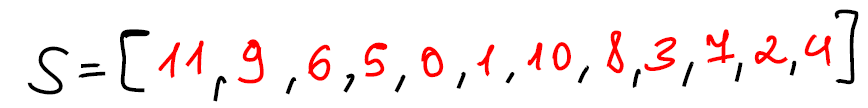
\includegraphics[width=0.4\textwidth]{images/state_image.PNG}
\caption{Initial random state}
\end{figure}
This state means that the facility number 11 is in location 0, facility 9 is in location 1 ... \\\\
Transitions are simply a swap of two facilities between two locations, so from the random state $s$ we could have a transition that would change the position of the facility 11 with the facility 9, this transition would be represented by $T(0,1) \longrightarrow$  we change the facility at location 0 with the facility at location 1, which results in $s'$\\\\
Let's see the effect of this transition in the state $s$:
\begin{figure}[H]
\center
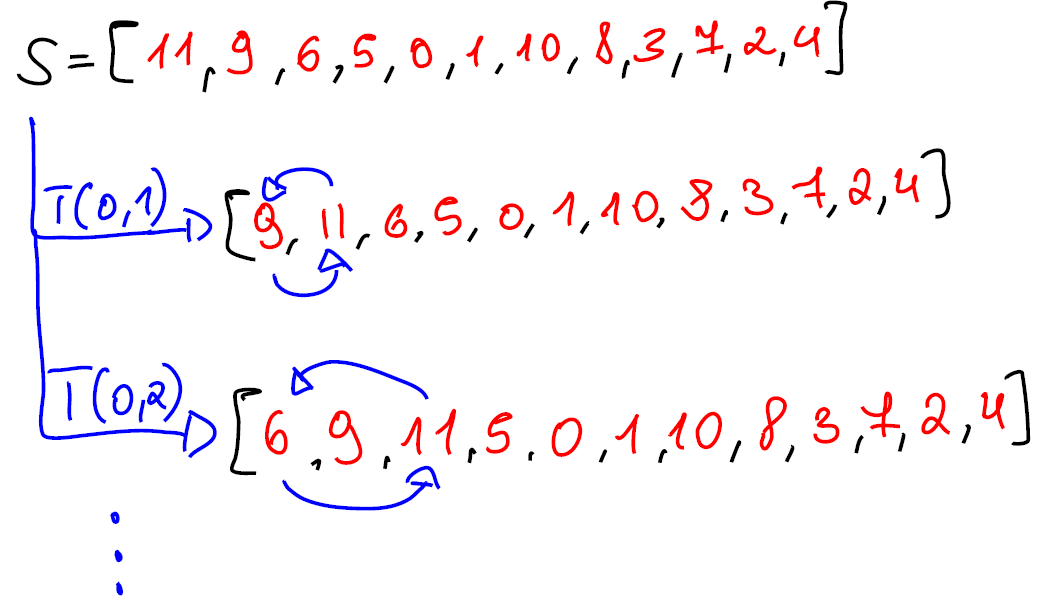
\includegraphics[width=0.6\textwidth]{images/state_transition.PNG}
\caption{Effect of T(0,1) and T(0,2) onto initial state $s$}
\end{figure}
This also means that at each step we have at least $ \sum_{i=1}^{n-1} $ transitions.\\\\
Suppose that the best transition is T(0,1), let's see how it will affect the Tabu List.\\
As we start the algorithm we initialize an array : $tabu\_list$ of size $(n \times n)$ full of zeroes. To update the $tabu\_list$ according to the transition T(0,1), we have to set $T_{s[0],0} = L$ and $T_{s[1],1} = L$, this means that the facility in $s[0]$ was in position $0$ $L$ iterations ago, and we want to block a transition that would place facility $s[0]$ in position $0$ for the next $L$ iterations.\\\\
Since we want to be able to place $s[0]$ in position $0$ in $L$ iterations, we have to update the values in $tabu\_list$ at each iteration: $$\textbf{if}\ (tabu\_list_{i,j} > 0) \textbf{ then : } tabu\_list_{i,j} = tabu\_list_{i,j} - 1 $$\\

This use of the $tabu\_list$ is the short item memory of the algorithm, but TS also has a variation that uses a long term memory to try and force transitions, as oppose to the short term memory that prevents some transitions.\\\\

The variation is called the diversification mechanism, this variation forces transitions that haven't been done in a $U$ iterations, just like $tabu\_list$ prevents transitions that were done $L$ iterations ago. In the same way we initialise $tabu\_list$ at the start of the algorithm, we also start a second array $diver\_list$ of size $(n \times n)$ full of zeroes. Each time we are trying to compute the neighbourhood of a given state, we first check if $diver\_list_{i,j} = U$ if we find such a value in $diver\_list_{i,j}$, then we force any transition that would place facility $i$ into position $j$. This helps the algorithm get unstuck or discover new horizons, after doing a forced transition, we set $diver\_list_{i,j} = 0$. We have to update $diver\_list$ at each iteration just like we did $tabu\_list$, so at each iteration:
$$\textbf{if}\ (tabu\_list_{i,j} < U) \textbf{ then : } diver\_list_{i,j} = diver\_list_{i,j} + 1 $$\\
We set $U = n^{2}$.
\begin{figure}[H]
\center
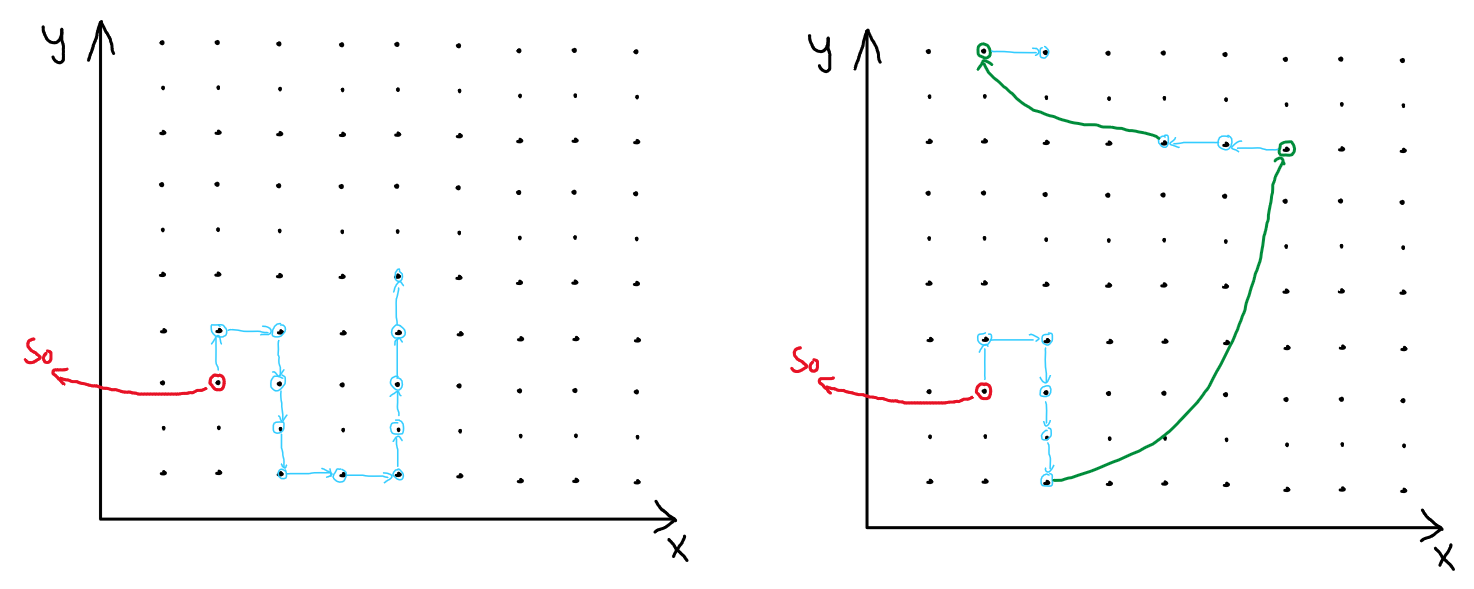
\includegraphics[width=1\textwidth]{images/with_without.PNG}
\caption{Exploration of $Z^{2}$ plane, left without diversification, right with diversification}
\end{figure}

The blue transitions are simple transitions from a state to it's close neighbour, and the green transitions symbolise a jump due to the diversification method.
\section{Results}

To test our algorithm and its variant we will implement what was explained in the previous section, and execute it 10 times with 20000 iterations, for each value of $L = \{1,6,10\}$ as well as with and without the use of the $diver\_list$. Before seeing the results I must say that I expect the use of $diver\_list$ to boost our results, as it will allow us to get unstuck from certain areas of the search space.

Let's first see the fitness found for each settings, we will only consider the best value of each setting in the table: \\
(first column is the best fitness of the 10 executions, second column is the average of the best fitnesses of the 10 executions, third column is the average fitness of the 20000 iterations in the best run, forth column is the max fitness - min fitness of the best run)
\begin{center}
Table 1 : Without Diversification\\
\begin{tabular}{|c|c|c|c|c|}
\hline
&    best fitness   & average best fitnesses     &  average fitnesses   & max-min    \\ \hline
L = 1   & 664   & 737  & 664.0   & 22   \\ \hline
L = 6  & 684  & 730  & 694.2  & 54   \\ \hline
L = 10 & 684 & 737 & 727.6 & 74 \\ \hline
\end{tabular}
\end{center}
\begin{center}
Table 2 : With Diversification\\
\begin{tabular}{|c|c|c|c|c|}
\hline
&    best fitness   & average best fitnesses     &  average fitnesses   & max-min    \\ \hline
L = 1   & 680   & 719  & 720.2   & 186   \\ \hline
L = 6  & 654  & 711  & 704.4  & 184   \\ \hline
L = 10 & 678 & 728 & 749.5 & 212 \\ \hline
\end{tabular}
\end{center}

The results aren't as I expected them, they show that the best settings were $L=6$ with the use of diversification, however I did expect a bigger difference in result. We see that on average the results with the use of diversification are better, but they best results aren't that much better than those without diversification.\\\\
I think this can be explained by looking at the last column of the table, we see that with the use of diversification, we explore much worse states, as the max-min is much larger, which means that the diversification method can lead us in the wrong direction, to compensate that we should increase the number of iterations. Diversification simply assures us that the search isn't located around the initial random state as it can be seen in Figure 3 from the previous section.

\end{document}
